%Copyright 2014 Jean-Philippe Eisenbarth
%This program is free software: you can 
%redistribute it and/or modify it under the terms of the GNU General Public 
%License as published by the Free Software Foundation, either version 3 of the 
%License, or (at your option) any later version.
%This program is distributed in the hope that it will be useful,but WITHOUT ANY 
%WARRANTY; without even the implied warranty of MERCHANTABILITY or FITNESS FOR A 
%PARTICULAR PURPOSE. See the GNU General Public License for more details.
%You should have received a copy of the GNU General Public License along with 
%this program.  If not, see <http://www.gnu.org/licenses/>.

%Based on the code of Yiannis Lazarides
%http://tex.stackexchange.com/questions/42602/software-requirements-specification-with-latex
%http://tex.stackexchange.com/users/963/yiannis-lazarides
%Also based on the template of Karl E. Wiegers
%http://www.se.rit.edu/~emad/teaching/slides/srs_template_sep14.pdf
%http://karlwiegers.com
\documentclass{scrreprt}
\usepackage{tikz}
\usepackage{listings}
\usepackage{underscore}
\usepackage[bookmarks=true]{hyperref}
\usepackage[utf8]{inputenc}
\usepackage[english]{babel}
\usepackage{pgfgantt}
\usepackage{CJKutf8}
\hypersetup{
    bookmarks=false,    % show bookmarks bar?
    pdftitle={Software Requirement Specification},    % title
    pdfauthor={Jean-Philippe Eisenbarth},                     % author
    pdfsubject={TeX and LaTeX},                        % subject of the document
    pdfkeywords={TeX, LaTeX, graphics, images}, % list of keywords
    colorlinks=true,       % false: boxed links; true: colored links
    linkcolor=blue,       % color of internal links
    citecolor=black,       % color of links to bibliography
    filecolor=black,        % color of file links
    urlcolor=purple,        % color of external links
    linktoc=page            % only page is linked
}%
\def\myversion{1.0 }
\date{}
%\title
\usepackage{hyperref}
\begin{document}
\begin{CJK}{UTF8}{bkai}
\begin{flushright}
    \rule{16cm}{5pt}\vskip1cm
    \begin{bfseries}
        \Huge{開放平台\\期末報告}\\
        \vspace{2.5 cm}
        $<$柯B$>$\\
        \vspace{2.5 cm}
        \LARGE{成員:}\\
        \vspace{1.0cm}
        范喻成\\
        \vspace{0.5cm}
        陳識允\\
        \vspace{0.5cm}
        黃柏凱\\
        \vspace{0.5cm}
        張哲家\\
        \vspace{0.5cm}
        \today\\
    \end{bfseries}
\end{flushright}

\tableofcontents

\chapter*{Revision History}

\begin{center}
    \begin{tabular}{|c|c|c|c|}
        \hline
	    Name & Date & Reason For Changes & Version\\
        \hline        
	    哲家 & 2018/6/15 & 把heroku上面的資料連結到github & 1\\
        \hline        
	    柏凱 & 2018/6/15 & 新增查詢電影的功能加入 & 2\\
        \hline
	    柏凱 & 2018/6/15 & 修復查詢電影的bug & 3\\
        \hline
	    柏凱 & 2018/6/15 & 新增requirements.txt的需求軟件 & 4\\
        \hline
	    識允 & 2018/6/15 & 新增youtube功能 & 5\\
        \hline
	    喻成 & 2018/6/15 & 新增latex和基本介紹 & 6\\
        \hline
	    哲家 & 2018/6/16 & 排版 & 7\\
        \hline
	    哲家 & 2018/6/17 & 新增翻譯功能 & 8\\
        \hline
	    哲家 & 2018/6/18 & 翻譯debug & 9\\
        \hline
	    識允 & 2018/6/18 & 更新youtube功能和新增help & 10\\
        \hline
	    哲家 & 2018/6/18 & bug fixed & 11\\
        \hline
	    哲家 & 2018/6/19 & 新增portal查詢作業與查氣象功能 & 12\\
        \hline
	    哲家 & 2018/6/19 & 修改requirements bug & 13\\
        \hline
	    識允 & 2018/6/19 & 修改氣象和翻譯 & 14\\
        \hline
	    哲家 & 2018/6/19 & portal改良 & 15\\
        \hline
	    哲家 & 2018/6/19 & bug fixed & 16\\
        \hline
	    哲家 & 2018/6/20 & portal防呆 & 17\\
        \hline
	    喻成 & 2018/6/20 & 更新latex & 18\\
        \hline
	    柏凱 & 2018/6/20 & 新增latex_ppt & 19\\
        \hline
	    識允 & 2018/6/20 & latex_ppt新增background & 20\\
        \hline
	    哲家 & 2018/6/21 & bug fixed & 21\\
        \hline
	    柏凱 & 2018/6/21 & 新增latex_ppt的設計理念與語意分析介面 & 22\\
        \hline
	    喻成 & 2018/6/21 & 修正latex & 23\\
        \hline
	    喻成 & 2018/6/21 & latex新增圖片 & 24\\
        \hline
	    識允 & 2018/6/21 & 新增latex的commit版本 & 25\\
        \hline
    \end{tabular}
\end{center}

\chapter{Introduction}

\section{Purpose}
此文件的目主要在於說明「柯B」這個產品所規劃的各項功能之特色、使用方式及參考文件,並介紹軟硬體的介面和目標客群。使用者可透過參考此份文件來了解本系統的架構、環境、作業流程, 可作為日後軟體設計與軟體測試的依據。

\section{Document Conventions}
文件中的Line bot以LB做簡稱。

\section{Intended Audience and Reading Suggestions}
本文件是為了開發人員、測試人員、使用者編寫。開發人員可以藉由此文件同步開發進度,測試人員及使用者可藉由此文件了解產品的理念以及使用方法。想要快速了解這個機器人的話,建議先去Part 4看看有甚麼功能,也別忘了去Part 5了解有關安全性的問題,以免發生錯誤。

\section{Project Scope}
我們LB希望可以達到產業合作的目標,透過我們的LB去結合其他公司的產品來達到合作,一方面為自己的團隊創造知名度另一方面也為該公司的新產品達到宣傳的目的,而該公司也可以省下聘請技術人員的成本,而產品維護的麻煩也可以避免,達到雙贏的局面。如果貴公司有單獨的願景,請參考本程式而不是直接複製程式。

\section{References}
{\color{blue}https://technews.tw}\\
{\color{blue}http://translate.google.com}\\
{\color{blue}https://movies.yahoo.com.tw}\\
{\color{blue}https://www.youtube.com}\\
{\color{blue}https://www.cwb.gov.tw}\\
{\color{blue}https://portalx.yzu.edu.tw}\\
{\color{blue}https://yaoandy107.github.io/line-bot-tutorial/}\\
{\color{blue}https://msdn.microsoft.com/zh-tw/library/dd409377.aspx}\\


\chapter{Overall Description}

\section{Product Perspective}
ChatBot最近流行一時,因為它可以根據特定的話語,產生不同的反應,如果設計良好,也可以帶來不少娛樂性以及便利性。於是我們想在Line上面實作出一個ChatBot(Line Bot),可以幫助使用者透過Line輕鬆查詢資料,省去不斷切換查詢頁面的麻煩。除此之外,因為我們身為學生需要時常確認課頁資訊,而一直登入portal很麻煩,因此我們想要讓LB可以幫助我們快速登入學校的porta取得想要的資訊。

\section{Product Functions}
1.  最新電影查詢\\
2.  可愛動物圖片查詢\\
3.  時事新聞查詢\\
4.  YouTube搜尋\\
5.  portal作業查詢\\
6.  氣象查詢\\
7.  中英翻譯\\

\section{User Classes and Characteristics}
我們的主要用戶是以學生為主,主要是因為我們的portal功能僅限元智學生可以登入使用,而我們的其他功能則是所有有需求者都是可以使用的,所以除了學生以外沒有特別區分使用者類別。此外我們程式有對用戶進行驗證是否為此系統的使用者,避免他人從外部要求做指令。

\section{Operating Environment}
硬體方面我們要求至少要有Line,而在手機板或電腦版都是可以接受的。除此之外沒有嚴格的軟硬體要求,只要能在電腦、手機上安裝Line並且透過Line ID或QR code加成好友便能使用我們的功能。

\section{Design and Implementation Constraints}
1.  資金: 對我們產品開發最大的約束可能就是錢,因為LB的主動推送訊息是需要錢才能使用的,而我們也沒有足夠的經費去啟用這功能,導致我們的LB能開發的功能大大的減少。\\
2.  伺服器: 因為金錢的關係,我們的產品只能選擇架設在免費的伺服器heroku上面,導致我們的LB有時候接受訊息再回復時會顯得非常遲緩。\\
3.  隱私: 我們的portal登入功能有涉及到帳號密碼的部分,所以加密以及保密顯得非常重要,這是我們需要去處理的問題。\\


\section{User Documentation}
由於我們的程式在操作方面算是非常簡單的,所以目前尚未設計所謂的User Documentation,僅有程式內部的內建help,而將來我們可能也會考慮架設一個可以及時幫助到客戶的線上客服系統,如此以來客戶在操作與使用我們的軟體時會更加輕鬆,也可以及時解決我們程式出現的bug,並在第一時間幫助到客戶,以提高我們的使用率。

\section{Assumptions and Dependencies}
1.  因為系統會藉由API、網頁取得資料,穩定的網路狀態是必須的。\\
2.  我們的機器人是建立在Line上,所以必須要預先安裝Line這個App。\\


\chapter{External Interface Requirements}

\section{User Interfaces}
因為是針對Line做的機器人,所以使用者介面大多是基於Line的聊天室介面,基本功能都可以直接在這個介面上透過點擊執行,而我們也有新增了help的按鈕在聊天室的底部,透過點擊help圖示可以得到我們所有功能的指令列表。\\
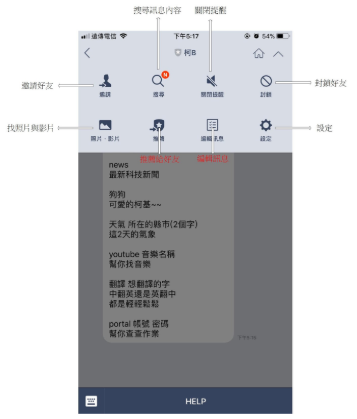
\includegraphics[width=8cm,height=10cm]{help1.png}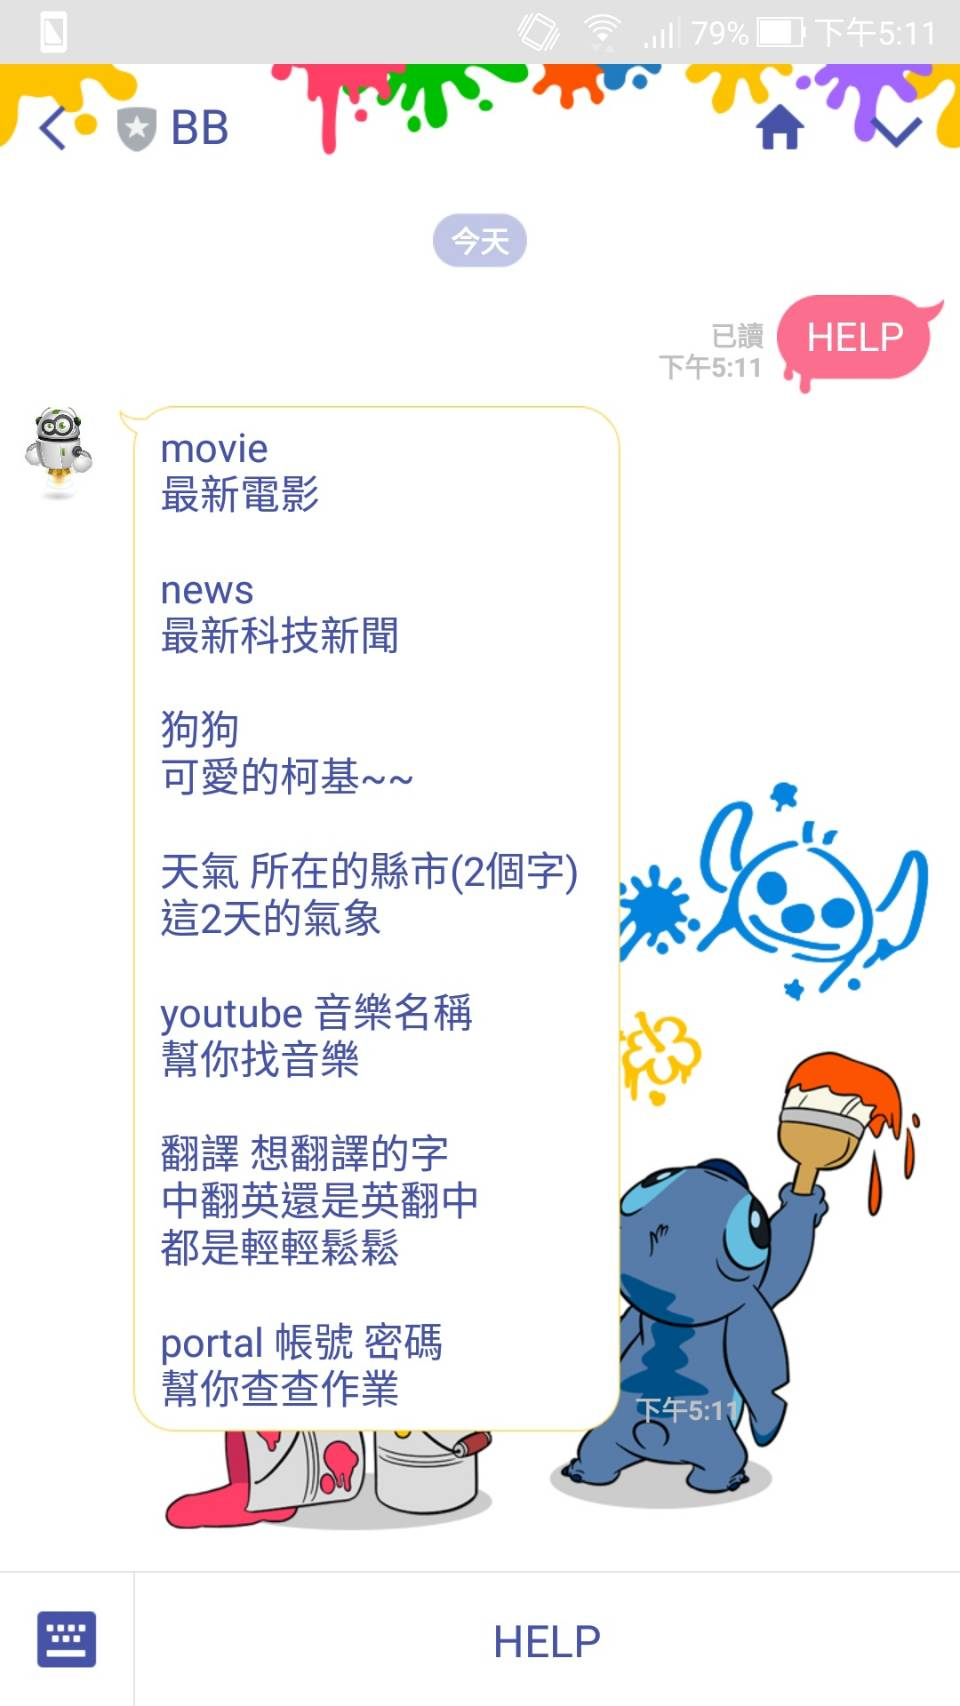
\includegraphics[width=8cm,height=10cm]{help2.png} 

\section{Hardware Interfaces}
無硬體介面

\section{Software Interfaces}
1.  主要使用Python語言來建置專案以及設定檔\\
2.  linebot套件與LinebotAPI做連接\\
3.  requests、bs4套件抓取網頁資訊\\
4.  urllib套件與API交換資料\\
5.  selenium套件模擬開啟網頁\\
6.  imgurpython套件連接imgur相簿\\

\section{Communications Interfaces}
1.  我們的專案必須鋪署在https協定的網域上,確保我們的程式是安全的\\
2.  我們抓取的資料須透過有SSL協定的管道來傳輸資料\\
3.  使用webdriver模擬開啟瀏覽器\\
4.  LINE使用LEGY通訊協定,除了能增加傳遞速度也能加強安全性\\


\chapter{System Features}

\section{電影、新聞、youtube查詢、翻譯}

\subsection{Description and Priority}
輕鬆取得最新電影、新聞、以及youtube的音樂等資訊,還可以翻譯單字\\
Priority: Low

\subsection{Stimulus/Response Sequences}
1.  輸入電影、新聞的相關詞彙,系統會到相關網站取得相關的標題及網址給使用者\\
2.  輸入youtube以及想要搜尋的視頻,系統會到youtube取得相關視頻資料前3筆給使用者\\
3.  輸入翻譯以及欲翻譯的詞彙,系統會回傳譯文給使用者\\

\subsection{Functional Requirements}
使用者必須依照格式輸入指令,格式錯誤會回傳無法辨識指令。\\
REQ-1: 使用者能在不用切換頁面的情況下查詢資料,節省時間。\\
REQ-2: 在群組聊天時能夠輕鬆分享資訊。\\
TBD-1: 增強語意辨識的能力。\\

\section{相簿功能}

\subsection{Description and Priority}
可以透過相簿取得特定照片\\
Priority: Low

\subsection{Stimulus/Response Sequences}
輸入動物相關詞語,系統會從相簿中隨機抓取一張相關照片回傳。\\

\subsection{Functional Requirements}
使用者必須依照格式輸入指令,格式錯誤會回傳無法辨識指令。\\
REQ-3: 使用者能在不用切換頁面的情況下取的照片,節省時間。\\

\section{天氣查詢}

\subsection{Description and Priority}
取得天氣資訊\\
Priority: Medium\\

\subsection{Stimulus/Response Sequences}
輸入天氣以及欲查詢的地區,系統會回傳目標地區的近2天溫度、天氣狀況、降雨機率等資料給使用者。\\

\subsection{Functional Requirements}
目前只能查詢台灣縣市範圍的天氣資訊,輸入以外的查詢內容會跳出錯誤提示。\\
REQ-4: 使用者可以迅速方便且正確的查詢天氣資訊。\\
TBD-2: 更細的地區查詢,例如: xxx 鄉/鎮/市。\\

\section{元智portal登入}

\subsection{Description and Priority}
登入學校portal取得作業資訊\\
Priority: High\\

\subsection{Stimulus/Response Sequences}
輸入portal以及帳號密碼,系統會登入學校portal取得作業資訊給使用者。\\

\subsection{Functional Requirements}
若輸入錯誤的帳號密碼,系統會提示登入失敗。\\
REQ-5: 使用者可以藉由簡單的指令取得portal的個人資料。\\
TBD-3: 提供使用者的課表、活動等相關資訊。\\

\chapter{Other Nonfunctional Requirements}

\section{Performance Requirements}
由於我們的功能大多是抓取網頁上的資訊,所以若當抓取網頁資訊的演算法過於複雜,可能會導致回傳資料給使用者的時間變長,因此我們主要以簡短又有效的方式抓取要求的資訊。

\section{Safety Requirements}
1.  限制用戶依定時間內對系統功能的要求次數$\rightarrow$避免類似DDOS的攻擊癱瘓系統。\\
2.  避免使用全域變數$\rightarrow$避免使用者更改到此變數進而影響系統。\\

\section{Security Requirements}
1.  必須驗證使用者發訊的來源是否來至本產品$\rightarrow$避免外人由外部操作本產品。\\
2.  須對重要的隱私訊息做隱藏$\rightarrow$由於有查詢portal的功能,所以密碼應受到隱藏,避免遭他人容易竊取資料功能。\\

\section{Software Quality Attributes}
1.  可測試性高: 輸入訊息後對照查詢的資料源可以很明顯看出回覆是否正確。\\
2.  易用性高: 只需要學會簡單的指令輸入就可以用。\\

\section{Business Rules}
For 團隊開發:\\
1.  團隊內部任何程式大型更動均需經過團隊半數以上同意才得以進行。\\
2.  團隊內部有任工作上緊急困難,其他人都需要立即幫助該同學盡快排解問題。\\
3.  程式任何push均需建立branch,經過審核通過才可merge入master。\\
4.  若程式有任何問題大家要盡速處理。\\
5.  若文檔有問題須優先處理。\\
6.  團隊互相輔助扶持,共創佳績!!!\\\\
For 使用:\\
1.  必須要有LINE的帳號。\\
2.  須將我們的機器人設為好友。\\
3.  若要使用portal功能需有portal帳號。\\
4.  用戶應可以隨時移除我們的機器人。\\
5.  用戶應知道LINE操作介面。\\

\chapter{Other Requirements}

\section{Appendix A: Glossary}
LEGY是LINE公司利用Erlang開發語言改寫SPDY協定所產生的,主要改善SPDY協定的延遲,因為LINE公司把LEGY協定設為一個主要通道,可以讓訊息先加密並快速傳送減少傳遞時間與增加安全。

\section{Appendix B: Analysis Models}
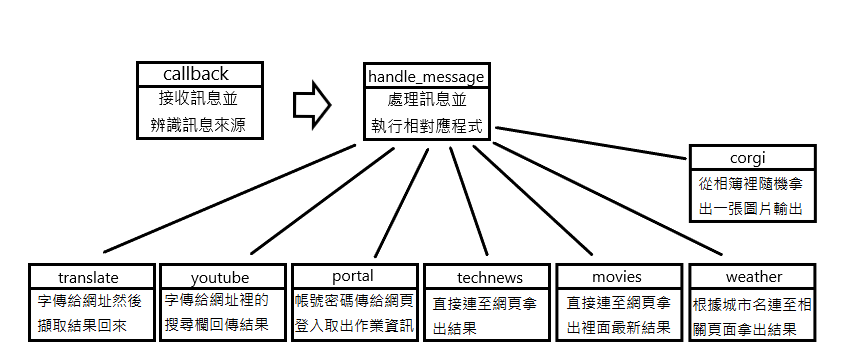
\includegraphics[width=16cm,height=10cm]{flow.png}

\section{Appendix C: To Be Determined List}
\begin{center}
    \begin{tabular}{|c|c|}
        \hline
	    TBD & 內容\\
        \hline        
	    1 & 增強語意辨識的能力。\\
        \hline        
	    2 & 更細的地區查詢,例如: xxx 鄉/鎮/市。\\
        \hline
	    3 & 提供使用者的課表、活動等相關資訊。\\
        \hline
    \end{tabular}
\end{center}

\end{CJK}
\end{document}